\documentclass{article}
\usepackage[]{ctex}

\usepackage{listings}

\title{LSM Tree实验报告}
\author{徐惠东 519021910861 }
\date{6月7日 2021年}

\usepackage{natbib}
\usepackage{graphicx}
\usepackage{enumitem}
\begin{document}

\maketitle

\section{背景介绍}
LSM Tree 全称 Log-structured Merge Tree, 是一种专门为 key-value 存储系统设计、可以高性能执行大量写操作
的数据结构。本项目是基于 LSM Tree 开发的一个简化的键值存储系统, 将用到跳表和sstable等数据结构,主要支持以下三种操作:
\begin{itemize}
    \item [1)] 
    PUT(K,V): 设置键 K 的值为 V       
    \item [2)]
    GET(K): 读取键 K 的值
    \item [3)]
    DELETE(K): 删除键 K 的值
\end{itemize}

% \begin{figure}[h!]
% \centering
% \caption{The Universe}
% \label{fig:universe}
% \end{figure}

\section{挑战}
\subsection{设计}
好的设计是成功的起点,也是代码实现简洁高效的必要前提。
遗憾的是,直到我快写完整个project我才体会到这句话的深刻含义。
项目开始前,我通读了近十遍ppt描述和pdf文档要求,对$LSM\_Tree$总体有了
大致的认识,随着项目不断进行,我也在不断修改和完善自己的代码结构。\par

1. 我将$KV\_Store$系统分为内存和磁盘两个部分,设计$KV\_Store$类如下,
其中$timestamp$维护一个全局的时间戳,正常启动时读取硬盘中文件最大时间戳并赋值,默认为1。
\begin{lstlisting}[language = C++, numbers=left, 
  numberstyle=\tiny,frame=single]
class KVStore : public KVStoreAPI {
private:
    uint64_t timestamp; // 时间戳
    /* 缓存的SSTable */
    std::vector<std::vector<SSTable*>> cache_MemTable;
    /* 当前的内存存储 */
    MemTable* cur_MemTable;
    /* 文件管理及合并器 */
    FileManager* fileManager;

    uint64_t max_size = 2 * 1024 * 1024; // 文件限制
    const std::string dir; // 写入文件夹
}
\end{lstlisting}

2. 根据面向对象设计原则,我将内存部分包装成一个类$MemTable$,内部用
跳表实现。
\begin{lstlisting}[language = C++, numbers=left, 
  numberstyle=\tiny, frame=single]
class MemTable {
private:
    Skiplist<uint64_t, std::string>* realize;
    uint64_t size;
}
\end{lstlisting}

3. 缓存部分即$SSTable$单独设计一个类,且$SSTable$可以直接作为写入
磁盘的中转类,而将$SSTable$中$DataArea$清空便可以作为缓存在内存的类,一举两用。
\begin{lstlisting}[language = C++, numbers=left, 
  numberstyle=\tiny,frame=single]
class SSTable
{
public:
  std::string filepath; // 文件名称
  struct Header {
      /* 共占用32B,用于存放元数据 */
      uint64_t timestamp;
      uint64_t key_value_num;
      uint64_t key_min;
      uint64_t key_max;
  } *_header;
  struct BloomFilter {
    public:
      /* 每个hash值为128-bit
       * 分为四个无符号32位整型使用
       */
      std::vector<std::vector<uint8_t>> _hash_table;
  } *_bloom_filter;
  struct IndexArea {
      /* 索引区,用来存储有序的索引数据
       * 包含所有的键及对应的值在文件中的offset
       * 占用 key_value_num * 12B
       */
    IndexData* _index;
  } *_index_area;
  struct DataArea {
    /* 数据区,用于存储数据(不包含对应的key)*/
    std::vector<std::string> _value;
  } *_data_area;
};
\end{lstlisting}

4. 对于$compaction$操作,由于其和内存、缓存以及磁盘都相关,最初是想设计在$KV\_Store$中实现,
但考虑到解耦合的重要性,便单独设计$FileManager$类进行$compaction$操作。
\begin{lstlisting}[language = C++, numbers=left, 
  numberstyle=\tiny,frame=single]
class FileManager {
  /* 将内存跳表转换成硬盘SSTable形式 */
  SSTable* memTableToSSTable(MemTable* Memtable,
                             uint64_t timestamp);
  /* 写入文件至硬盘 */
  std::string writeFileToDisk(...);
  /* 从硬盘中读取文件至缓存 */
  SSTable* getOneFileFromDisk(std::string filepath, 
                              bool emptyDataArea);
  /* 合并操作 */
  void compaction(std::set<std::string>& add_cache,
                  std::set<std::string>& del_cache);
}
\end{lstlisting}

\subsection{困难与挑战}
我在做LSM Tree Project中遇到了许多困难,小的困难包括删除指针前没有检查非空指针、
数据区存储方式选择等,这些问题往往能在debug后发现并及时解决。然而,在整个项目过程
中,我也遇到了一些令我烦躁的、较为难以解决或者需要大改代码的问题,简述如下:
\begin{itemize}
    \item [1)] 
    由于缺乏大型的项目代码经验和忽视内存释放的代码习惯,使得我在内存释放上显得力不从心。以至于当数据量变大时,内存直接爆炸,为此
    我在后期花费了大量时间和精力用于寻找内存泄漏的位置。\\
    最终发现是在跳表删除结点时漏掉了近一半的结点,因此每次使用跳表时便会多出
    很多的垃圾内存,导致内存泄漏问题。还有我使用了stl库中的vector存放临时字符串,经过上网搜索发现clear()函数无法完全释放vector
    所用全部内存,必须使用.swap()函数才可以。\\
    经过认真修正这些问题后,我的程序已经几乎不存在内存泄漏的问题(当然不能保证百分百)。
    这也让我深深地意识到内存管理的重要性、以及及时手动释放无用内存的必要性。       
    \item [2)]
    文件命名的问题同样困扰着我。对于每一层文件夹的命名没有什么争议,即以$level-0$代表第0层,以此类推。
    对于每一层文件夹中小文件命名,最初我的设计是$'SSTable-' + timestamp$来命名,并直接由文件名对应时间戳,这样每次
    读文件便可以获取对应时间戳。\\
    但当我开始写合并时就发现时间戳可能因为合并而相等,所以两个文件的名字会相同,这在文件系统中当然是不允许的。
    为了修复这个bug,我只能在缓存SSTable中加入时间戳这一变量用来记录时间戳,而文件命名时则在后面继续加入数字以解决重名
    覆盖问题。当读取文件至缓存中时,保存相应文件名和时间戳,用来一一对应缓存的SSTable和实际的文件。
    \item [3)]
    在进行合并时,我会从最高层(0层)-> 最底层(n层)依次检测,如果该层没有超出该层文件数量限制,那么后面所有层
    都不会超出对应层文件数量限制,则直接跳出检测并返回。如果超出,则将超出的文件向下读入缓存后删除文件,在将下一层
    中与这些文件有键值范围交集的文件读入缓存后删除文件,在内存中对键值进行排序(排序方式:键值小的优先,相同键值时间戳大的优先,相同
    键值相同时间戳的层数靠上的优先),并直接将键值对转换为相应的文件写入硬盘,再进行下一层的检测。检测完后对所改变的文件夹层所对应的
    缓存进行修改。
\end{itemize}

\section{测试}
\subsection{测试环境}
\begin{itemize}[align = left]
  \item [机型] LG 14Z990-V.AA52C
  \item [处理器] Intel(R) Core(TM) i5-8265U CPU \@ 1.60GHz(8 CPUs), ~1.8GHz
  \item [内存] 8192MB RAM
  \item [磁盘驱动器] SAMSUNG MZNLN256HAJQ-00000
\end{itemize}
\subsection{性能测试}

\subsubsection{预期结果}

\begin{itemize}
    \item [GET] 
    内存中查找:内存使用跳表存储键值对,单次查找操作的平均时间复杂度为 O(log n)。\\
    硬盘中查找:先在缓存中查找,因为每个缓存都有布隆过滤器,所以仅需 O(1) 即可判断是否在该 SSTable 中,
    判定存在后使用二分查找找到 offset,平均时间复杂度也为 O(log n)。因此 Get 操作
    的平均时间复杂度是 O(log n) 其中 n 为平均每个 SSTable 所容纳的键值对个数。 \\
    但实际上硬盘读写速度远小于内存读写速度,因此对于访问硬盘的 Get 操作,硬盘读写应占到了绝大多数时间。
    \item [PUT]
    不发生归并:不发生归并时,仅在跳表中插入该键值对,先搜索跳表,查找该元素,这一步
    需要 O(log n) 的时间,然后执行插入,因为跳表每一元素期望的塔高为2,因此可以在常
    数时间内完成插入。\\
    发生归并:具体的时间花费与数据的区间、硬盘中已经存在的数据分布情况有关。
    但发生归并会因为进行多次文件读写,时间消耗巨大。
    \item [DEL]
    先执行 Get 操作,如果找到再执行 Put 操作插入一条"\~{}Delete\~{}",因此其期望耗时
    应为 Get 与 Put 的期望耗时之和,但实际上因为插入的字符仅占 8 个字符,发生归并的概率
    不高,因此其实际时间消耗应小于 Get 与Put 时间消耗之和。
\end{itemize}

\subsubsection{常规分析}
Get、Put、Delete 操作的延迟与吞吐结果如表 \ref{figure1} ,表 \ref{figure2} 所示。
在延迟部分的测试中,我分别测试了数据大小为256,512,1024,2048,4096, 9192 bytes 情况下三种操作的延迟,并计算出了均值。在吞吐量测试中,我
选取了数据大小为10240 bytes 的数据进行测试。 \par
可以看到,PUT 操作的效率会比 GET 操作和 DEL 操作慢较多,这是因为当put触发compaction时会
花费大量时间在文件读写上。而 DEL 操作和 GET 操作耗时随着数据量增加略有增加但相对稳定,
这是因为大多数操作都是先搜索布隆过滤器,如果查找到了则读取文件,否则直接返回空,因此数据量增大
对其延迟并没有直接大的影响。\par
DEL 操作稍慢于 GET 操作。DEL 操作相当于一次 GET 操作接着一次
PUT 操作,因此它相较于 GET 操作会慢一些;又由于 DEL 中存入的数据
很小("\~{}Delete\~{}"),因此它很少触发合并,没有 PUT 操作那么慢。
PUT 操作的大延迟与读写磁盘次数较多有关。\par

\begin{table}[h!]
    \begin{center}
      \caption{不同数据大小下PUT, GET, DEL 操作平均延迟}
      \label{figure1}
      \begin{tabular}{c|c|c|c}
        \textbf{数据大小/byte} & \textbf{PUT延迟/us} & \textbf{GET延迟/us} & \textbf{DEL延迟/us}\\
        \hline
        256 & 24.99 & 68.49 & 65.43 \\
        512 & 54.23 & 66.22 & 68.63 \\
        1024 & 80.26 & 54.54 & 61.79 \\
        2048 & 192.17 & 70.16 & 72.11 \\
        4096 & 453.92 & 68.41 & 73.12 \\
        9192 & 1136.98 & 63.46 & 67.44 \\
        \hline
      \end{tabular}
    \end{center}
\end{table}

\begin{table}[h!]
    \begin{center}
      \caption{数据大小为4096 bytes 时PUT, GET, DEL 操作的吞吐}
      \label{figure2}
      \begin{tabular}{c|c|c|c}
        \textbf{数据大小/byte} & \textbf{PUT吞吐/$s^{-1}$} & \textbf{GET吞吐/$s^{-1}$} & \textbf{DEL吞吐/$s^{-1}$}\\
        \hline
        4096 & 102439 & 67842 & 19981 \\ 
      \end{tabular}
    \end{center}
\end{table}

\subsubsection{索引缓存与Bloom Filter的效果测试}
不同缓存情况下GET 操作的平均延迟结果如表3。
这里同样测试了数据大小为256,512,1024,2048,4196 bytes 情况
下三种缓存情况的延迟。需要注意的是在无缓存情况下,表中数据的单位是
ms。
这里的结果和前面的分析一样,没有缓存索引时GET 操作的延迟远远
大于缓存索引的延迟,在这个测试中相差了两个数量级左右;而缓存布隆过
滤器会提高GET 性能,但是提高的程度没有缓存索引带来的明显。

\begin{table}[h!]
    \begin{center}
      \caption{不同缓存情况下GET 操作平均延迟}
      \label{figure3}
      \begin{tabular}{c|c|c|c}
        \textbf{数据大小/byte} & \textbf{不缓存/ms} & \textbf{缓存索引/us} & \textbf{缓存索引与布隆过滤器/us}\\
        \hline
        256 & 70.28 & 59.93 & 66.02 \\
        512 & 57.81 & 66.57 & 50.30 \\
        1024 & 57.93 & 90.36 & 68.54 \\
        2048 & 74.64 & 99.24 & 90.88\\
        4096 & 71.06 & 77.24 & 59.55 \\
        \hline
        average & 66.34 & 78.67 & 67.09 \\ 
      \end{tabular}
    \end{center}
\end{table}

\subsubsection{Compaction的影响}
不断插入数据情况下PUT 操作的吞吐量结果如图~\ref{img}。
测试中为提高compaction 的频率,插入的数据大小为10KB,测试吞
吐量的时间间隔缩短为1000ms。\par
图中可以看出,包含compaction 的时间段中PUT 操作的吞吐量会不断下
降很多,这是符合预测的。

\begin{figure}
    \centering
    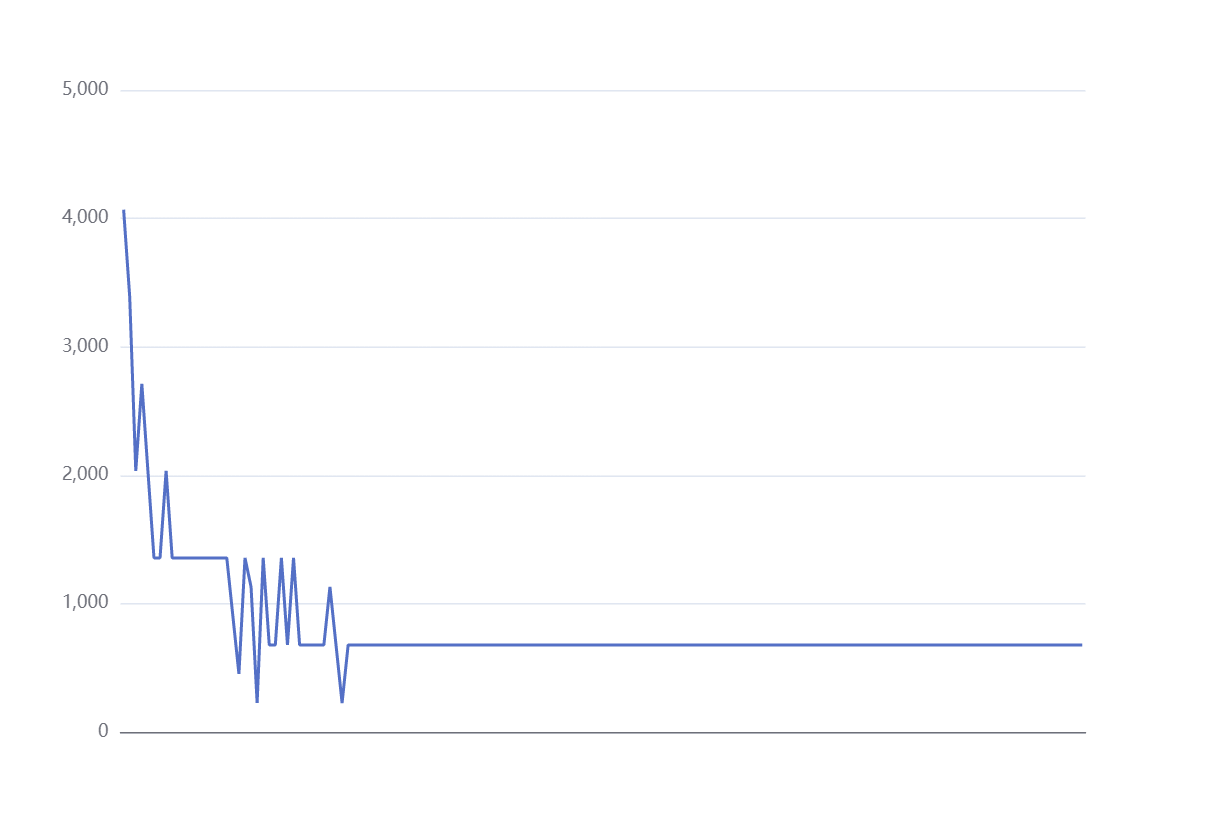
\includegraphics[width=.8\textwidth, height=6cm]{get_latency.png}
    \caption{合并测试} %caption是图片的标题
    \label{img} %此处的label相当于一个图片的专属标志,目的是方便上下文的引用
\end{figure}

\newpage
\section{体验与收获}
我平时喜欢在OJ上刷一些小题当做放松方式,OJ上的大多数题都是考验脑子转的快不快。
然而,我渐渐发现,要想成为一名优秀的程序员,更需要有提前规划的能力,不仅是提前规划
进度与安排,还有提前对代码结构进行规划,这一点只能通过完成一个个lab来不断提升。\par
尤其记得大一上的软件基础实践做第一个lab时,当时完全没有头绪还向助教请教如何提升这种提前
规划的能力,当时助教给我的答复便是多练,到现在我对这点已经深信不疑了。\par
这次的$LSM_Tree$不同于以往的project,它需要和文件读写打交道,而这一块正是我大一上几乎没有了解过的
内容,听往届的学长学姐的吐槽,感觉挑战性很大。\par
但真正做起来时,吸取上学期半死不活的贪吃蛇项目经验,我提前做了部分架构,规定了一些接口函数,
并从顶层往底层依次设计,将任务粗分为内存、磁盘及内存与磁盘的交互这几个部分,然后再不断细分成
各种函数,这样我便可以对接口编程了,也省去了各个函数集成的痛苦。\par
因此,在最初一个月内,我并没有感受到很大的压力,相反,我甚至没有对着二进制文件死磕,当文件读写出问题
时,我会先在内存中查找问题,或是将文件内容读入内存再寻找问题所在,而不是直接将二进制文件翻译成文本文件来
查看,这样也提升了我的效率。\par
到了后期,特别是和compaction打交道的时候,我开始变得有些难受,先是内存泄漏问题让我的程序根本运行不下去,
然后便是向下compaction的速度太慢,我都尽力解决了。对于这次project,我深刻体会到内存管理的重要性,以及提前做好代码整体架构重要性,而不是一上手就写代码,
这样返工成本太高。\par
非常感谢老师和助教设计出如此精妙、简洁而不简单的project,也非常感谢这一过程中助教的答疑解惑,让我最终能够顺利
地完成这次project,我收获很大,痛并快乐着。。\par
至于有什么建议,如果非要说出一两条,那我希望project的解释文档更加详细一些,以及规定一下最终运行测试代码的机器类型,
虽然我在windows和linux虚拟机里都跑成功了,但还是有点小慌。
\end{document}
